\documentclass{article}
\title{Relazione 3: Integrazione Numerica}
\author{Antonio Michele Miti}


\usepackage{amsmath}
\usepackage{amsfonts}
\usepackage[utf8]{inputenc}
\usepackage[italian]{babel}
\usepackage{listings}
\usepackage{textcomp}
\usepackage{graphicx}
\usepackage{subfigure}
\usepackage{rotating}
\usepackage{caption}
\usepackage{latexsym}
\usepackage{epstopdf}
\usepackage{eepic,epic,eepicemu}
\usepackage{color}
\pagestyle{headings}
\definecolor{listinggray}{gray}{0.9}
\definecolor{lbcolor}{rgb}{0.95,0.95,0.95}
\lstset{
	backgroundcolor=\color{lbcolor},
	rulecolor=,
	language=C++,
        basicstyle=\scriptsize,
        upquote=true,
        aboveskip={1.5\baselineskip},
        columns=fixed,
        showstringspaces=false,
        extendedchars=true,
        breaklines=true,
        prebreak = \raisebox{0ex}[0ex][0ex]{\ensuremath{\hookleftarrow}},
        frame=single,
        showtabs=false,
        showspaces=false,
        showstringspaces=false,
        identifierstyle=\ttfamily,
        keywordstyle=\color[rgb]{0,0,1},
        commentstyle=\color[rgb]{0.133,0.545,0.133},
        stringstyle=\color[rgb]{0.627,0.126,0.941},
}
\addtolength{\hoffset}{-1.25cm}
\addtolength{\voffset}{-1.80cm}
\addtolength{\textwidth}{1cm}
\addtolength{\textheight}{3.80cm}

\newtheorem{legge}{Definizione}

\begin{document}
\maketitle
\begin{abstract}
In questo articolo si intende studiare la convergenza di alcuni integrali numerici di funzioni su $\mathbb{R}$ al variare delle iterazioni utilizzate per calcolarlo. 

Si scelgono delle funzioni particolari per evidenziare la dipendenza della convergenza dei vari algoritmi dalle proprietà di regolarità della funzione integranda.

Gli algoritmi considerati sono esclusivamente non adattivi e vengono confrontati a parità di punti della funzione che vengono valutati, confrontare le iterazioni sarebbe scorretto in quanto ogni algoritmo valuta un set diverso di punti per iterazione.
Nei casi migliori si otterà una convergenza di $\frac{1}{a}$ con $a$ parametro dipedendente dal metodo usato.
\end{abstract}

%\tableofcontents

\section{Introduzione}

La maggior parte dei metodi di integrazione numerica si basa sugli stessi presupposti:  

partendo dall'integrale da calcolare $$I = \int_{a}^{b}f(x)dx$$ vengono scelti $x_{1},\ldots,x_{n}\in [a,b]$ punti nel intervallo di integrazione al fine di suddividere il calcolo dell'integrale iniziale in quello di un numero $K$ di integrali su intervalli più piccoli: 
	\begin{equation}
	\int_{a}^{b}f(x)dx= \sum_{n=0}^{K-1}\int_{x_{n}}^{x_{n+1}}f(x)dx = \sum_{n=0}^{K-1}I_{n}
	\end{equation}
dove $x_{0}=a$ e $x_{K}=b$.

L'approssimazione numerica risiede nel modo in cui viene stimata la quantità $I_{n}$.

I metodi di integrazione che verranno studiati sono tutti "non adattivi" ovvero i punti $x_{i}$ vengono scelti equispaziati da una distanza $h$. Sostanzialmente questo comporta che intorni dei punti critici e intervalli molto regolari vengano trattati tutti nello stesso modo.
Questo è ovviamente fonte di errori sistematici in modo strettamente dipendente dall'andamento delle funzioni di cui si vuole calcolare l'integrale ma ha il vantaggio di non richiedere alcuno studio preliminare delle proprietà dell'integranda.

\subsection{Metodo dei Rettangoli}

Sono i metodi di quadratura più semplici e derivano direttamente dalla definizione operativa di integrale di Riemman, ovvero consistono nell'approssimazione:
$$I \simeq I_{\textrm{sup}} \qquad I \simeq I_{\textrm{sup}} $$
Per fare questo è necessario costruire la polinomiale che approssima la funzione.
Avendo già un set di ${x_{n}}$ punti del dominio in cui campionare la funzione si costruisce la polinomiale come la funzione:
\begin{equation}
	\chi(x) = \left\{ 
			\begin{array}{l}
 			y=0 \qquad \textrm{con} x < x_{0}\\
 			y=0 \qquad \textrm{con} x > x_{K} \\
			y= f(x_{j}) \qquad \textrm{con} \qquad x_{j} \leq x < x_{j+1} \qquad (\textrm{rettangolo sinistro}) \\
  			\end{array} \right.
	\end{equation}

(Oppure $ y= f(x_{j+1})$ con $ x_{j} < x \leq x_{j+1}$, nel caso del rettangolo destro)

La definizione di integrabilità secondo Riemman implica che , valutando un numero $N$ di punti della funzione,il
$$  \lim_{N \rightarrow \infty}I_{\textrm{sup}}=\lim_{N \rightarrow \infty}I_{\textrm{sup}}=\int_{a}^{b}f(x)dx$$

Per cui l'integrale della polinomiale:
$$\int_{a}^{b}\chi(x)dx = \sum_{n=0}^{K-1}f(x_{n})(x_{n+1}-x_{n})$$
converge all'integrale della funzione $f(x)$ al crescere dei punti campionati (al tendere a zero dell'incremento), ed è approssimabile ad esso per un numero finito (grande) di punti.

Operativamente in tutto questo non si è fatto altro che approssimare il valore del integrale $I_{n}$ della formula (1) come un rettangolo:
\begin{equation}
			\begin{array}{l}
 			I_{n} \simeq  f(x_{n})(x_{n+1}-x_{n}) \qquad \textrm{rettangolo sinisto}\\
				o\\
 			I_{n} \simeq  f(x_{n+1})(x_{n+1}-x_{n}) \qquad \textrm{rettangolo destro}\\
			\end{array} 
	\end{equation}.

\subsection{Calcolo numerico degli integrali $I_{n}$}

Siano $I_{n}=\int_{a'}^{a'+h}f(x)dx$ gli integrali "infinitesimi" definiti precedentemente, é possibile il calcolo approssimato di questo quantità definendo il "Polinomio Interpolante di Lagrange":
	
\begin{legge}[Polinomio Interpolante di Lagrange]
	siano $a_{1},\ldots,a_{n} \in [a',a'+ h]$ N punti detti insieme di campionamento della funzione, allora:
    	\begin{equation}
		P(x)=\sum_{i=1}^{N}f(a_{i})\prod_{j \neq i}\dfrac{x-a_{j}}{a_{i}-a{j}}
		\end{equation}
	\end{legge}

Il polinomio così definito gode delle seguenti proprietà:

\begin{itemize}
\item[-] $P(x)$ è un approssimante di $f(x)$ : $\lim_{n\rightarrow\infty}P(x)=f(x)$
\item[-] $P(x)$ interseca f(x) nei punti $a_{i}$ di campionamento
	\begin{displaymath}
		\mu_{l}(x)=\prod_{j \neq l}\dfrac{x-a_{j}}{a_{l}-a{j}} = \left\{
			\begin{array}{ll}
			1 & \textrm{$x=a_{l}$}\\
			0 & \textrm{$x\neq a_{l}$}\\
 			\end{array} 
		\right.
	\end{displaymath}
\item[-] $P(x)$ è un polinomio di grado $N$ 
\end{itemize}

Quindi se poniamo $P(x)\simeq f(x)$ si ottiene
	\begin{equation}
	I_{k}\simeq\int_{a_{k}}^{a_{k}+h}P(x)dx= \sum_{i=1}^{n}f(a_{i})\omega_{i}
	\end{equation}
dove $\omega_{i}$ sono detti "coefficienti di peso" o più semplicemente "pesi"
	\begin{equation}
	\omega_{i}=\int_{a_{k}}^{a_{k}+h}\prod_{j \neq i}\dfrac{x-a_{j}}{a_{i}-a{j}}
	\end{equation}

I Pesi sono esattamente determinati dal modo in cui vengono scelti i punti appartenti all'insieme di campionamento $a_{1},\ldots,a_{n} \in [a',a'+ h]$.
I differenti metodi di approssimazione del integrale infinitesimo sono caratterizzati da due proprietà: il numero N dei punti di campionamento e la loro disposizione nel dominio di integrazione.
Tutto ciò è perfettamente consistente alla definizione di integrale di Riemman nel limite di $N\longrightarrow\infty$.

Si osserva inoltre che l'identità $P(x)=f(x)$ è esattamente vera fino al ordine di approssimazione N, quindi se suddividiamo l'intervallo di integrazione da cui siamo partiti ($[a,b]$) in un numero $K$ di intervallini sufficientemente grandi è lecito poter approssimare su di essi, con un errore modesto, la funzione $f(x)$ ai primi termini del suo sviluppo di Taylor.

\subsection{Metodi di Newton-Costes}

In questi metodi i punti di campionamento vengono sempre scelti in modo da suddividere l'intervallo iniziale $[a,b]$ in intervalli equispaziati. Questo implica nei sottointervalli infinitesimi il seguente schema di campionamento:

	\begin{displaymath}
		\begin{tabular}{lcccccccccr}
			&   & & $a_{k}$ & & & &$a_{k+1}$ &  &   &\\
			n=1 & &   & $\mid$ & & X & & $\mid$ & &   &\textrm{punto medio}\\
			n=2 & &   & X & & $\mid$ & & X & &   &\textrm{trapezi}\\
			n=3 & &   & X & & X & & X & &   &\textrm{simpson}\\
		\end{tabular} 
	\end{displaymath}
(la X indica dove cade il punto campionato nel sottointervalli $I_{n}$).

Questa tabella individua i primi 3 metodi di integrazione Newton-Costes. Da queste informazioni è possibile ricavarne i Pesi.

\paragraph{Metodo del Punto Medio}

Consiste nell'approssimazione del valore dell'integrale su un intervallo di ampiezza $h$ con l'area di un rettangolo di base $h$ ed altezza data dal valore di $f(x)$ nel punto medio dell'intervallo considerato.

	\begin{equation}
	I_{k}\simeq f(a_{k}+\frac{h}{2})h
	\end{equation}

Il metodo è esatto per le funzioni costanti e quelle lineari, di conseguenza l'approssimazione di una qualsiasi funzione sarà affetta da un errore dell'ordine $o(h)$.

\paragraph{Metodo dei Trapezi}

Consiste nell'approssimazione del valore dell'integrale su un intervallo di ampiezza $h$ con l'area di un trapezio di altezza $h$ e con basi date dai valori $f(x)$ agli estremi del intervallo.

	\begin{equation}
	I_{k}\simeq (f(a_{k})+f(a_{k}+h))\frac{h}{2}
	\end{equation}

Esattamente come il metodo precedente, l'approssimazione numerica è esatta per funzioni costanti e lineari,ovvero è valida per lo sviluppo di una qualsiasi funzione fino all'ordine $o(h)$.

Si osserva che ordine del approssimazione non coincide necessariamente con la precisione. L'ordine dice fino a che ordine, in senso analitico, la funzione è rappresentata da quello sviluppo, l'errore del metodo invece sarà la differenza tra il valore ottenuto numericamente e l'effettivo sviluppo analitico fino al dato ordine.

Quindi anche se i due metodi sono esatti fino allo stesso ordine non implica che siano efficienti computazionalmente allo stesso modo.

\paragraph{Metodo di Simpson}

Questo metodo è la generalizzazione dei risultati precedenti a 3 punti.
Supponendo di voler scrivere una formula di integrazione sull'intervallo $[x,x+h]$ che utilizzi solo il valore della funzione in 3 punti otterremo in generale un equazione del tipo:
	
\begin{equation}
	\int_{a_{k}}^{a_{k}+h}f(x)dx= h[af(a_{k})+bf(a_{k}+\frac{h}{2})+cf(a_{k}+h)]
	\end{equation}
dove a,b,c sono parametri incogniti.

Imponenendo che questa approssimazione sia esatta per tutte le funzioni fino al secondo ordine incluso qualsiasi sia il valore di $h$, ottengo le seguenti condizioni sui tre parametri.
\newline
Usando come prova per l'ordine 0 $f(x)=1$
	\begin{displaymath}
	\int_{x}^{x+h}dx=h=h[a+b+c]\Longrightarrow a+b+c=1
	\end{displaymath}
usando $f(x)=x$ come prova per il primo ordine: 
	\begin{displaymath}
	\int_{x}^{x+h}xdx=\dfrac{(x+h)^{2}-x^{2}}{2}=h[ax+b(x+\frac{h}{2})+c(x+h)]
	\end{displaymath}
	\begin{displaymath}
	\frac{h^{2}}{2}+xh= h(a+b+c)x+\frac{h^{2}}{2}(b+2c)\Longrightarrow
	\end{displaymath}
usando $f(x)=x^{2}$ come prova per il secondo ordine: 
	\begin{displaymath}
	\int_{x}^{x+h}x^{2}dx=\dfrac{(x+h)^{3}-x^{3}}{3}=h[ax^{2}+b(x+\frac{h}{2})^{2}+c(x+h)^{2}] \Longrightarrow \frac{8}{3}h^{2}=(b+4c)h^{3}\Rightarrow b+4c = \frac{8}{3}
	\end{displaymath}

In conclusione i parametri devono soddisfare il sistema di 
	\begin{displaymath}
		\left\{
			\begin{array}{l}
			a+b+c=1 \\
			b+2c=1 \\
			b+4c=\frac{4}{3}
 			\end{array} 
		\right.
	\end{displaymath}

Ovvero sia $D= \frac{h}{2}$ si ottiene l'espressione:
	\begin{equation}
	\int_{a_{k}}^{a_{k}+h}f(x)dx= D[f(a_{k})+4f(a_{k}+D)+f(a_{k}+2D)]
	\end{equation}

Quindi, partendo dal presupposto dell'esattezza del metodo fino all'ordine $n$ dello sviluppo, si possono ottenere in modo analogo a quanto fatto per Simpson (n=3) tutti gli altri ordini dei metodi di Newton-Costes.

\subsection{Metodi di Gauss}

Se si rilascia la condizione di equispaziotura dei punti di campionamento nell'intervallino si ottengono i metodi di quadratura di Gauss.

In generale, la filosofia che sta dietro la costruzione di tali algoritmi è la seguente: vengono scelti i pesi e lo schema di campionamento in modo che la relativa quadratura risulti esatta per una certa classe di funzioni del tipo:
$$f(x)=W(x)P(x) .$$

In altre parole dato $W(x)$ e un numero intero $N$, si cercano un set di pesi $\omega_{j}$ e un set di ascisse $x_{j} \in [a_{k},a_{k}+h]$ tali che l'approssimazione:
	\begin{equation}
	\int_{a_{k}}^{a_{k}+h}W(x)f(x)dx\simeq \sum_{j=1}^{N}f(a_{j})\omega_{j}
	\end{equation}
sia esatta quando $f(x)$ è un generico polinomio.

A questo punto cambiando notazione, definendo $g(x)=W(x)f(x)$ e $v_{j}=\omega_{j}/W(a_{j}$ si ottiene una forma esplicita della quadratura di gauss:
	\begin{equation}
	\int_{a_{k}}^{a_{k}+h}g(x)dx \simeq \sum_{j=1}^{N}g(a_{j})v_{j}
	\end{equation}
identica alla formula per la generica quadratura del polinomio di lagrange della funzione.

A questo punto basta utilizzare le coppie $[x_{j},v_{j}]$ già tabulate al variare di $N$ per una specifica scelta della funzione $W(x)$, (in questo caso vengono utilizzati i polinomi di legendre), per implementare l'algoritmo di questa quadratura.
Ci si aspetta che i metodi di quadratura di Gauss siano, a parità di punti di campionamento, più accurata dei vari metodi di Newton-Costes.

\subsection{Metodo Montecarlo}

Il metodo di Montecarlo è un metodo concettualmente diverso da quelli precedenti: è un metodo statistico, facilmente estendibile a funzioni a molte dimensioni ma applicabile solo su intervalli di integrazione in cui la funzione integranda rimane limitata.

Si consideri un supporto $[a,b]$ su cui la funzione integranda sia definita positiva, vengono scelti in modo casuale N punti nella regione rettangolare del piano $R^{2}$ che ha per base $[a,b]$ e ha per altezza il massimo della funzione su tale intervallo.
A questo punto è possibile stimare l'area sottesa dalla funzione come l'area del rettagolo per la frazione di punti casuali $(x,y)$ che si trovano all'interno della regione sotto la funzione, ovvero tali che $y \leq f(x)$.

\section{Metodologia}
Si realizzano in \emph{C++} gli appositi algoritmi per calcolare l'integrale numerico secondo ciascun metodo di integrazione descritto sopra lasciando come parametro arbitrario il numero $n$ di iterazioni utilizzate [ vedere file integrazione.h].
Nel file sono presenti due tipi di algoritmi, quelli per gli integrali impropri e quelli per gli integrali su intervalli finiti. In realtà non c'è nessuna differenza concettuale, il calcolo di qualsiasi quadratura richiede di fissare il parametro dell'ampiezza della campionatura (o, equivalentemente, del numero di punti valutati). 

Il calcolo dell'integrale su un intervallo illimitato richiede ulteriormente di dare un approssimazione dell'infinito, questa scelta è solitamente dettata dall'andamento della funzione e dalla rapidità della corvengenza.

A seconda del metodo di integrazione, per ogni iterazione la funzione verrà valutata in un numero differente di punti:

\begin{displaymath}		
		\begin{tabular}{|c|c|}
		\hline
		\textrm{Rettangoli} & 1 \\
		\textrm{Trapezi} & 2 \\
		\textrm{Simpson} & 3 \\
		\textrm{Gauss di ordine n} & n \\
		\hline
		\end{tabular} 
\end{displaymath}

In altre parole ogni metodo stima l'integralino $I_{k}$ valutando la funzione in un numero differente di punti.

Per i metodi di Newton-Costes con $n>1$ il numero di punti valutati è vero solo in senso computazionale, ovvero il computer valuta la variabile $f(x)$ ogni volta che viene chiamata nel ciclo, ma in senso analitico il numero di punti valutati è sempre minore di quello indicato. Questo perchè in tali metodi i punti vengono campionati sul bordo degli intervalli e intervalli consecutivi condividono lo stesso bordo. Si conclude che per $N$ iterazioni il metodo dei rettengoli valuta complessivamente $N$ punti, il metodo dei trapezi $N+1$ punti e il metodo di simpson $2N+1$ punti. 

A questo punto si stampa per ogni algoritmo (testandolo su differenti funzioni integrande) :
$$\mid I_{atteso}-I_{numerico}(n)\mid = f(n)$$
ovvero il  modulo della differenza tra il risultato del integrale atteso e quello numerico in funzione del numero dei punti valutati e si confrontano i grafici risultanti.

Quindi si esegue il fit dei grafici trovati rispetto una funzione del tipo:
$$f(x)=x^{A}$$
il coefficiente A darà l'ordine del errore del algoritmo.

\newpage
\section{Casi di Studio}

Facendo i grafici si dimostra che il valore esatto del errore dipende direttamente dalle proprietà della funzione si cui vengono applicati gli algoritmi, funzioni con molte oscillazioni o con derivate molto grandi richiedono più punti per essere correttamente risolte con metodi numerici.
Lista delle funzioni studiate:
\paragraph{Funzione A}
	\begin{equation}
	f_{A}(x)=\dfrac{1-\cos(2x)}{x^{2}}
\qquad
	\int_{0}^{\infty}f_{A}(x)=\pi
	\end{equation}
\begin{figure}[h]
	\centering
	\caption{Funzione A}
	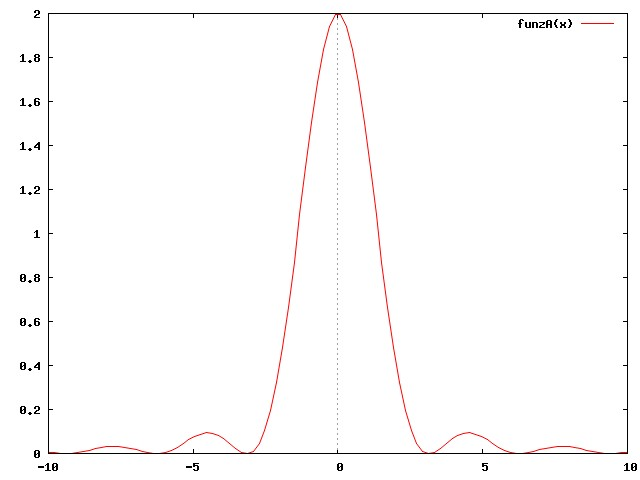
\includegraphics[width=5cm,,keepaspectratio]{pictures/funzA.jpg}
	\end{figure}

Particolarità di questa funzione è la forma d'indecisione $\frac{0}{0}$ nel origine e la convergenza dell'integrale indefinito.La forma d'indecisione non permette di calcolare il valore esattamente sullo zero, quindi è necessario approssimare il punto iniziale con $0+\varepsilon$.

\paragraph{Funzione B}
	\begin{equation}
	f_{B}(x)=\dfrac{1}{\sqrt{25-x^{2}}}
	\qquad
	\int_{0}^{5}f_{B}(x)=\frac{\pi}{2}
	\end{equation}

\begin{figure}[h]
	\centering
	\caption{Funzione B}
	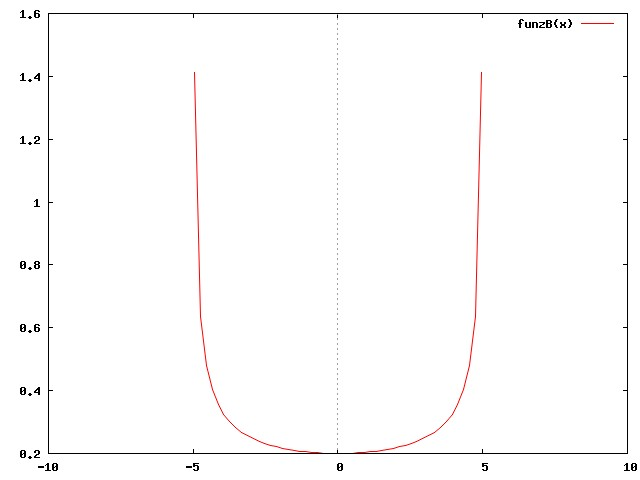
\includegraphics[width=5cm,,keepaspectratio]{pictures/funzB.jpg}
	\end{figure}

Questa funzione è definita reale solo nel intervallo $[-5,5]$ e presenta degli asintoti verticali agli estremi del intervallo di definizione. Come prima il valore al bordo non è computazionalmente definito quindi e necessario porre $5-\varepsilon$ come estremo destro dell'integrale.


\paragraph{Funzione C}
	\begin{equation}
	f_{C}(x)=\sin(x)
	\qquad
	\int_{0}^{\pi}f_{C}(x)=2
	\end{equation}

\begin{figure}[h]
	\centering
	\caption{Funzione C}
	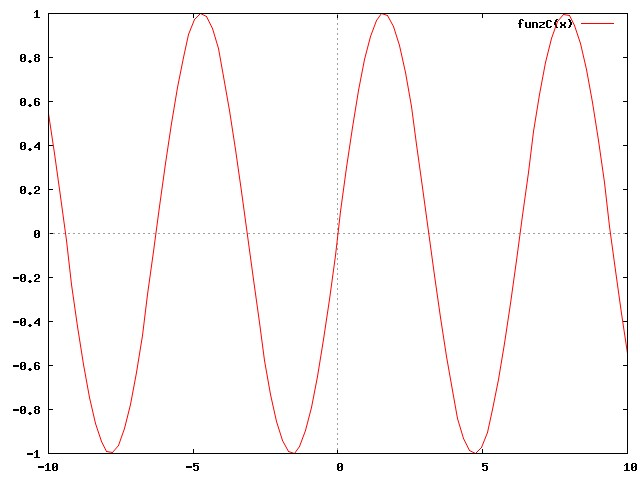
\includegraphics[width=6cm,,keepaspectratio]{pictures/funzC.jpg}
	\end{figure}

E' una funzione regolare con una crescita lenta e definita su tutto $\Re$. Gli algoritmi non dovrebbero trovare nessuna difficoltà a computare questo integrale.


\paragraph{Funzione D}
	\begin{equation}
	f_{D}(x)=\exp-(x^{2}+\frac{1}{x^{2}})
	\qquad
	\int_{0}^{\infty}f_{D}(x)=\frac{\sqrt{\pi}}{2}e^{2}
	\end{equation}

\begin{figure}[h]
	\centering
	\caption{Funzione D}
	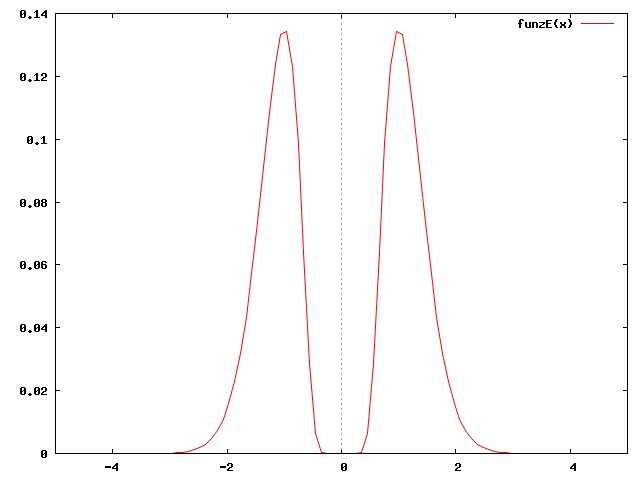
\includegraphics[width=6cm,,keepaspectratio]{pictures/funzE.jpg}
	\end{figure}

Una funzione evanescente limitata superiormente su tutto il dominio che tende a 0 molto rapidamente, è sostanzialmente diversa da 0 solo in un piccolo intervallo $[0,5]$.

\paragraph{Funzione E}
	\begin{equation}
	f_{E}(x)=\dfrac{\log(x)}{1+x}
	\qquad
	\int_{0}^{1}f_{E}(x)=-\frac{\pi^{2}}{12}
	\end{equation}

	\begin{figure}[h]
	\centering
	\caption{Funzione E}
	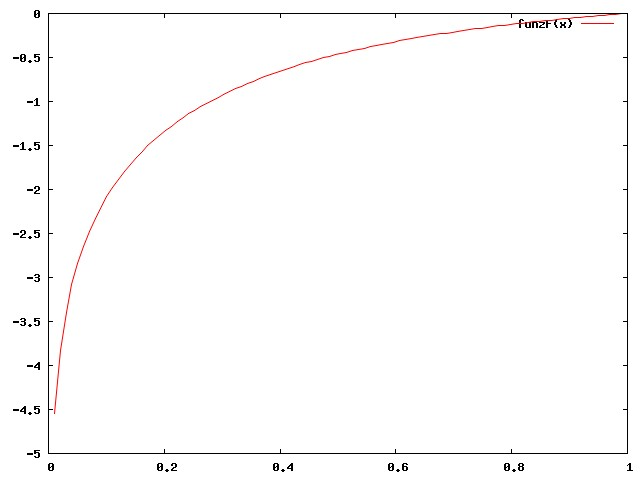
\includegraphics[width=6cm,,keepaspectratio]{pictures/funzF.jpg}
	\end{figure}

Funzione non definita in 0 che ammette comunque integrale indefinito, semplice modifica della funzione D quindi soffre della stessa approssimazione intorno all'origine.

\clearpage
\section{Risultati}
\paragraph{Funzione A}

Sampando contmporaneamente i grafici dei risultati per tutti i metodi si nota , come previsto, che gli integrali convergono al valore vero (a meno della necessaria approssimazione di $\infty\simeq 250$) al crescere del numero dei punti campionati.

Il problema è che l'andamento della convergenza oscilla in modo irregolare quindi non è possibile stimare il modo in cui decresce. 
	\begin{figure}[h]
	\centering
	\caption{Confronto quadrature $f_{A}$}
	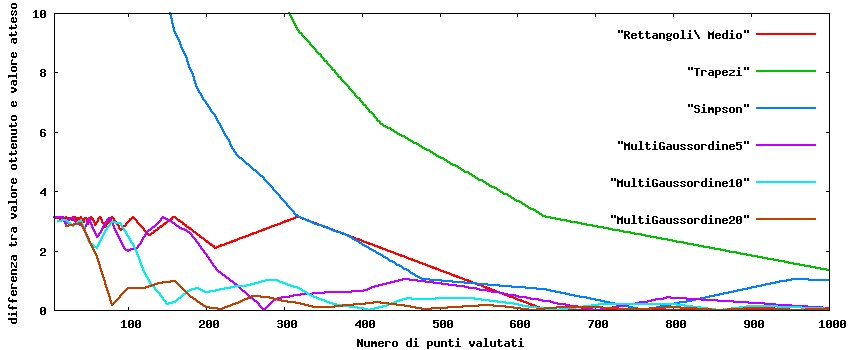
\includegraphics[width=13cm,,keepaspectratio]{pictures/funzA/confronto.jpg}
	\end{figure}

In generale si nota una approssimazione migliore, a parità di punti, con i metodi di Gauss rispetto a quelli di Newton. Questa condizione non è universalmente vera, infatti il valore calcolato tramite il metodo dei rettangoli nel punto medio, quando i punti valutati superano i 600, smette di oscillare e comincia decrescere in modo monotono presentando un accordo molto migliore rispetto agli altri metodi.

\paragraph{Funzione B}

Da un primo confronto qualitativo degli andamenti delle quadrature si nota che i metodi di Newton con $n>1$ presentano l'errore maggiore.
	
\begin{figure}[h]
	\centering
	\caption{Confronto quadrature $f_{B}$}
	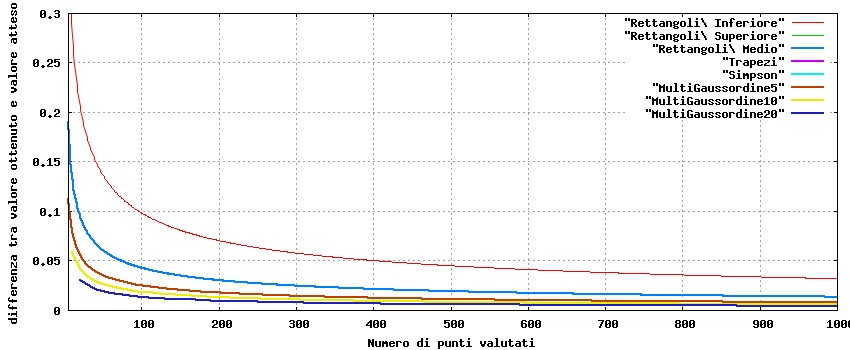
\includegraphics[width=13cm,,keepaspectratio]{pictures/funzB/confronto.jpg}
	\end{figure} 

Questo è dovuto al fatto che tali metodi valutano la funzione sempre al bordo degli intervallini quindi l'elevata pendenza implica che l'incremento delle ordinate sia molto grande in proporzionale a quello delle ascisse.
 
L'elevata concavità inoltre fa si che la funzione tenda ad appoggiarsi maggiormente sulla base del rettangolo inferiore rispetto a quella del superiore, per questo i metodi del rettangolo superiore e del punto di mezzo si dimostrano più efficienti rispetto agli alti metodi di newton che valutano la funzione nel punto più alto.
Per lo stesso motivo i metodi di Gauss ,che non valutano mai la funzione al bordo dell'intervallo, sono particolarmente efficienti.

I grafici sono sufficientemente regolari per fare un fit polinomiale dei punti tramite \emph{gnuplot}.
Usando come funzione di fit $f(x) = C + B x^{-A}$ si ottengono i valori:

\begin{tabular}{|c|l|l|c|}
\hline
metodo & A & B & $\chi^{2}_{\textrm{rid}}$ \\
\hline \hline
Ret inf 	   & 0.43688 $\pm$ 4.19e-04 & 0.77478 $\pm$ 8.55e-04 & 3.413e-07\\
\hline
Ret Med        & 0.49938 $\pm$ 9.81e-06 & 0.42614 $\pm$ 2.04e-05 & 3.295e-10\\
\hline
gauss V ordine & 0.49965 $\pm$ 8.29e-06 & 0.25013 $\pm$ 5.32e-06 & 2.713e-12\\
\hline
gauss X ordine & 0.49989 $\pm$ 3.70e-06 & 0.18537 $\pm$ 1.95e-06 & 8.673e-14\\
\hline 
gaus XX ordine & 0.49998 $\pm$ 2.05e-06 & 0.13430 $\pm$ 8.65e-07 & 3.744e-15\\ 
\hline

\end{tabular}
\\

I coefficienti C non sono considerati, rappresentano un errore causato principalmente dall'approssimazione dell'estremo di integrazione $5$ con $5-\varepsilon$, risultano comunque dell'ordine del $10^{-6}$ quindi completamente trascurabili.

In conclusione si osserva che l'errore decresce secondo la stessa potenza ($\frac{1}{N^{\frac{1}{2}}}$) nonostante i diversi metodi siano analaliticamente precisi ad ordini dello sviluppo di taylor progressivamente crescente.

\paragraph{Funzione C}

La funzione presa in considerazione è estremamente regolare, questo implica che i metodi con precisione maggiore (i metodi di gauss) abbiano un valore di incertezza prossimo alla precisione macchina.

I valori si dispongono quindi a strati, a distanza finita in prossimità dello zero($\sim 1o^{-8}$) rendendo impossibile l'analisi dell'andamento.

	\begin{figure}[h]
	\centering
	\caption{Confronto quadrature $f_{C}$ tra 0 e $\pi$}
	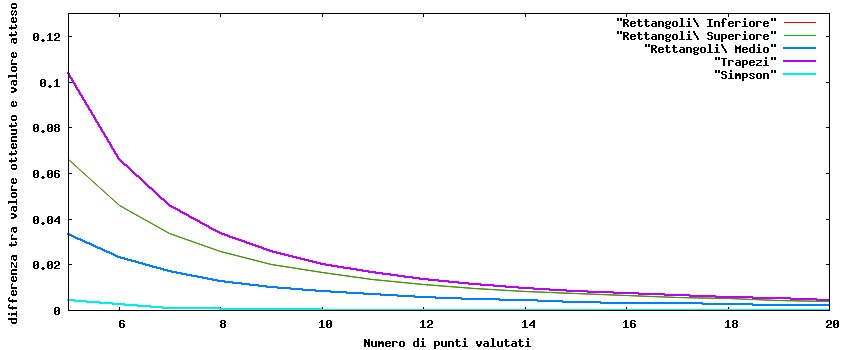
\includegraphics[width=13cm,,keepaspectratio]{pictures/funzC/confronto.jpg}
	\end{figure}


\paragraph{Funzione D}

Questo caso è un lampante esempio dell'irregolarità del incertezza a seconda della complessità della funzione integranda.
	\begin{figure}[h]
	\centering
	\caption{Confronto quadrature $f_{D}$ con $\infty \simeq 5000$}
	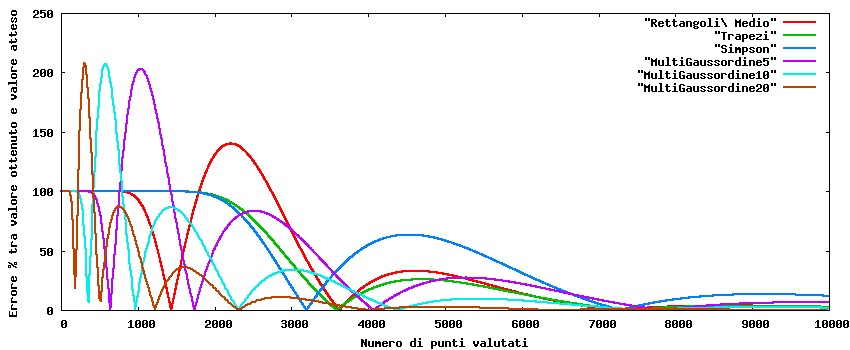
\includegraphics[width=13cm,,keepaspectratio]{pictures/funzE/confronto.jpg}
	\end{figure}

Il vero problema nell'integrazione numerica di questa funzione sta nella scelta opportuna del valore approssimante $\infty$. La funzione è praticamente diversa da zero solo per un piccolo intervallo della retta $\Re$ vicino all'origine, quindi ponendo l'infinito molto avanti l'algoritmo necessiterà di molte iterazioni per arrivare a valutare la funzione laddove è diversa da 0. 

Per questo il grafico di tutti gli algoritmi presenta inizialmente una parte rettilinea dovuta al fatto che gli $N$ punti valutati non cadono mai nel supporto della funzione e l'integrale risulta praticamente nullo.
Per lo stesso motivo gli andamenti oscillano smorzando progressivamente l'ampiezza (garantendo l'annullarsi dell'errore all'infinito).	
	
\begin{figure}[h]
	\centering
	\caption{Confronto quadrature $f_{D}$ con $\infty \simeq 10$}
	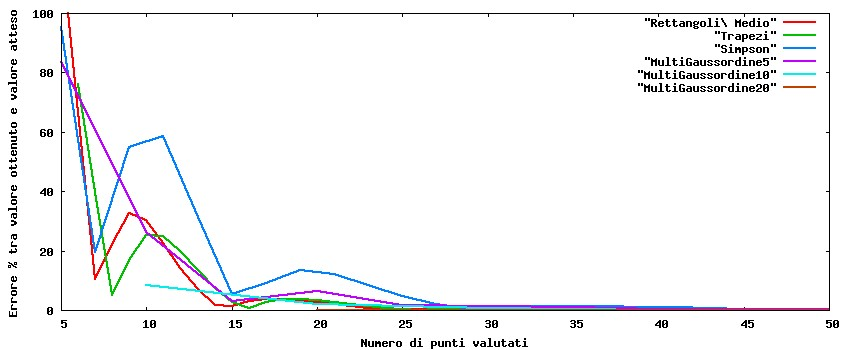
\includegraphics[width=13cm,,keepaspectratio]{pictures/funzE/confronto2.jpg}
	\end{figure}

Si può provare a compensare a questo tipo di errore riducendo l'intervallo di integrazione, ovvero approssimando l'infinito ad un valore più piccolo.

Come si nota dal secondo grafico la convergenza di tutti i metodi è molto più rapida in questo modo, tutti gli algoritmi risultano più efficienti al prezzo di un maggiore errore sistematico nel considerare nulla la funzione dopo l'estremo. Errore che si può stimare numericamente caso per caso. 

Per questa funzione vale, sul bordo destro, che $$f(\infty)=e^{-(10^{2}+10^{-2})} \sim e^{-(100)} \simeq 10^{-100}$$ in altre parole per tutte le ascisse maggiori di 10 la funzione assume un valore estremamente piccolo, totalmente fuori dalla portata delle precisione della macchina.

\paragraph{Funzione E}

La funzione è regolare e anche in questo caso i metodi di Gauss risultano di gran lunga più efficienti degli altri algoritmi di quadratura.
	\begin{figure}[h]
	\centering
	\caption{Confronto quadrature $f_{E}$}
	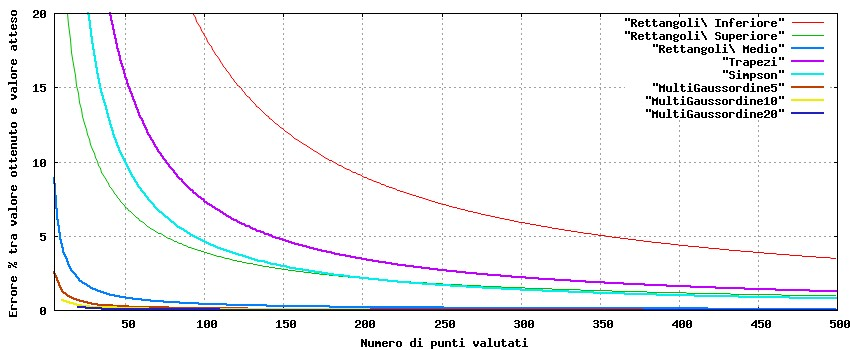
\includegraphics[width=13cm,,keepaspectratio]{pictures/funzF/confronto.jpg}
	\end{figure}

Per quando riguarda i metodi di Newton invece, anche in questo caso il metodo di ordine 1 risulta più efficace degli ordini superiori. 

La motivazione è sempre la solita, gli algoritmi di newton risentono particolarmente della concavità della funzione negli intervalli in cui la derivata prima è , in valore assaluto, elevata.

Dal grafico è evidente la grande concavità, la veloce crescita della funzione deriva necessariamente dal polo nell'origine per il quale nell'intervallo $[0,1]$ la funzione assume valori tra $[-\infty,0]$.

I grafici sono sufficientemente regolari per fare un fit polinomiale della dispersione tra valore ottenuto e valore atteso in funzione del numero dei punti tramite \emph{gnuplot}.

Usando come funzione di fit $f(x) = C + B x^{-A}$ si ottengono i valori:

\begin{tabular}{|c|l|l|c|}
\hline
metodo & A & B & $\chi^{2}_{\textrm{rid}}$ \\
\hline \hline
Ret Med        & 1.02116 $\pm$ 1.69e-04 & 0.37729 $\pm$ 1.40e-04 & 2.345e-10\\
\hline
trapezi		   & 1.17206 $\pm$ 1.47e-03 & 12.0493 $\pm$ 4.06e-02 & 5.636e-06\\
\hline
simpson        & 1.12932 $\pm$ 6.80e-04 & 6.7363  $\pm$ 0.013 & 1.176e-07\\
\hline
gauss V ordine & 1.00617 $\pm$ 1.04e-04 & 0.10747 $\pm$ 2.42e-05 & 4.138e-12\\
\hline
gauss X ordine & 1.00161 $\pm$ 2.58e-05 & 0.05778 $\pm$ 4.20e-06 & 1.866e-14\\
\hline 
gaus XX ordine & 1.00051 $\pm$ 4.75e-06 & 0.03013 $\pm$ 5.00e-07 & 4.344e-17\\ 
\hline

\end{tabular}
\\

Da cui si nota che tutti i metodi decadano a zero come $\dfrac{1}{N}$ ma con efficienza differente, la stessa osservabile qualitativamente sul grafico.

\section{Conclusione}

Dall'analisi precedente si è evideziato la dipendenza della convergenza del metodo di integrazione numerica dalla regolarità della funzione integranda.

I metodi di Newton ne risentono maggiormente, in sistabza i metodi di Gauss si dimostrano quelli computazionalmente più efficienti in tutti i casi presi in considerazione.




\begin{thebibliography}{99}
\bibitem{recipe}\emph{Numerical recipes in C++}
\bibitem{knuth}Knuth D. \emph{The Art of Computer Programming}
\bibitem{hilde}Hildebrand F. \emph{Introduction to Numerical Analysis}, 2nd.ed.
\end{thebibliography}
\end{document}


\paragraph{Funzione D}
	\begin{equation}
	f_{D}(x)=\lg (x)
	\qquad
	\int_{1}^{a}f_{D}(x)=a\lg(a)-a+1
	\end{equation}

